\documentclass[11pt,]{article}
\usepackage[left=1in,top=1in,right=1in,bottom=1in]{geometry}
\newcommand*{\authorfont}{\fontfamily{phv}\selectfont}
\usepackage[]{mathpazo}


  \usepackage[T1]{fontenc}
  \usepackage[utf8]{inputenc}



\usepackage{abstract}
\renewcommand{\abstractname}{}    % clear the title
\renewcommand{\absnamepos}{empty} % originally center

\renewenvironment{abstract}
 {{%
    \setlength{\leftmargin}{0mm}
    \setlength{\rightmargin}{\leftmargin}%
  }%
  \relax}
 {\endlist}

\makeatletter
\def\@maketitle{%
  \newpage
%  \null
%  \vskip 2em%
%  \begin{center}%
  \let \footnote \thanks
    {\fontsize{18}{20}\selectfont\raggedright  \setlength{\parindent}{0pt} \@title \par}%
}
%\fi
\makeatother




\setcounter{secnumdepth}{0}

\usepackage{longtable,booktabs}

\usepackage{graphicx,grffile}
\makeatletter
\def\maxwidth{\ifdim\Gin@nat@width>\linewidth\linewidth\else\Gin@nat@width\fi}
\def\maxheight{\ifdim\Gin@nat@height>\textheight\textheight\else\Gin@nat@height\fi}
\makeatother
% Scale images if necessary, so that they will not overflow the page
% margins by default, and it is still possible to overwrite the defaults
% using explicit options in \includegraphics[width, height, ...]{}
\setkeys{Gin}{width=\maxwidth,height=\maxheight,keepaspectratio}

\title{\textbf{The effect of \emph{Ascophyllum nodosum} extracts on plant
productivity and fungal and bacterial communities.}  }



\author{\Large Sébastien Renaut\textsuperscript{1,2},Jacynthe
Masse\textsuperscript{1,2}, Mengxuan Kong\textsuperscript{1,2}, Mohamed
Hijri\textsuperscript{1,2}\vspace{0.05in} \newline\normalsize\emph{\textsuperscript{1}Département de Sciences Biologiques, Institut de
Recherche en Biologie Végétale, Université de Montréal, 4101 Sherbrooke
Est, Montreal, H1X 2B2, Quebec, Canada. \textsuperscript{2}Quebec Centre
for Biodiversity Science, Montreal, Quebec, Canada}  }


\date{}

\usepackage{titlesec}

\titleformat*{\section}{\normalsize\bfseries}
\titleformat*{\subsection}{\normalsize\itshape}
\titleformat*{\subsubsection}{\normalsize\itshape}
\titleformat*{\paragraph}{\normalsize\itshape}
\titleformat*{\subparagraph}{\normalsize\itshape}





\newtheorem{hypothesis}{Hypothesis}
\usepackage{setspace}

\makeatletter
\@ifpackageloaded{hyperref}{}{%
\ifxetex
  \PassOptionsToPackage{hyphens}{url}\usepackage[setpagesize=false, % page size defined by xetex
              unicode=false, % unicode breaks when used with xetex
              xetex]{hyperref}
\else
  \PassOptionsToPackage{hyphens}{url}\usepackage[unicode=true]{hyperref}
\fi
}

\@ifpackageloaded{color}{
    \PassOptionsToPackage{usenames,dvipsnames}{color}
}{%
    \usepackage[usenames,dvipsnames]{color}
}
\makeatother
\hypersetup{breaklinks=true,
            bookmarks=true,
            pdfauthor={Sébastien Renaut\textsuperscript{1,2},Jacynthe
Masse\textsuperscript{1,2}, Mengxuan Kong\textsuperscript{1,2}, Mohamed
Hijri\textsuperscript{1,2} (\textsuperscript{1}Département de Sciences Biologiques, Institut de
Recherche en Biologie Végétale, Université de Montréal, 4101 Sherbrooke
Est, Montreal, H1X 2B2, Quebec, Canada. \textsuperscript{2}Quebec Centre
for Biodiversity Science, Montreal, Quebec, Canada)},
             pdfkeywords = {Stella Marris, 16S, ITS, microbial diversity, Illumina MiSeq},  
            pdftitle={\textbf{The effect of \emph{Ascophyllum nodosum} extracts on plant
productivity and fungal and bacterial communities.}},
            colorlinks=true,
            citecolor=blue,
            urlcolor=blue,
            linkcolor=magenta,
            pdfborder={0 0 0}}
\urlstyle{same}  % don't use monospace font for urls

% set default figure placement to htbp
\makeatletter
\def\fps@figure{htbp}
\makeatother

\usepackage[left]{lineno}
\linenumbers


% add tightlist ----------
\providecommand{\tightlist}{%
\setlength{\itemsep}{0pt}\setlength{\parskip}{0pt}}

\begin{document}
	
% \pagenumbering{arabic}% resets `page` counter to 1 
%
% \maketitle

{% \usefont{T1}{pnc}{m}{n}
\setlength{\parindent}{0pt}
\thispagestyle{plain}
{\fontsize{18}{20}\selectfont\raggedright 
\maketitle  % title \par  

}

{
   \vskip 13.5pt\relax \normalsize\fontsize{11}{12} 
\textbf{\authorfont Sébastien Renaut\textsuperscript{1,2},Jacynthe
Masse\textsuperscript{1,2}, Mengxuan Kong\textsuperscript{1,2}, Mohamed
Hijri\textsuperscript{1,2}} \hskip 15pt \emph{\small \textsuperscript{1}Département de Sciences Biologiques, Institut de
Recherche en Biologie Végétale, Université de Montréal, 4101 Sherbrooke
Est, Montreal, H1X 2B2, Quebec, Canada. \textsuperscript{2}Quebec Centre
for Biodiversity Science, Montreal, Quebec, Canada}   

}

}








\begin{abstract}

    \hbox{\vrule height .2pt width 39.14pc}

    \vskip 8.5pt % \small 

\noindent The abstract will be written here


\vskip 8.5pt \noindent \emph{Keywords}: Stella Marris, 16S, ITS, microbial diversity, Illumina MiSeq \par

    \hbox{\vrule height .2pt width 39.14pc}



\end{abstract}


\vskip 6.5pt


\noindent \doublespacing \newpage 

\section{INTRODUCTION}\label{introduction}

Liquid extracts of marine macroalga are used as biostimulants in
agriculture. These extracts contain phytohormones that can influence
physiological processes even at very low concentrations (Craigie 2011).
Stella Maris® is derived from fresh \emph{Ascophyllum nodosum} harvested
from the nutrient-laden waters of the North Atlantic off the Eastern
Coast of Canada.\\
\hspace*{0.333em}\\
The aim of this project was to develop a better understanding of the
effects of \emph{A. nodosum} extracts on plant growth. We tested the
effect of these extract on two commonly used plants (Tomato -
\emph{Solanum lycopersicum} and Pepper - \emph{Capsicum annuum}) using
different measures of productivity. In addition, we tested how the
bacterial and fungal communities responded to the addition of \emph{A.
nodosum} extracts.\\
\hspace*{0.333em} ~

\section{MATERIAL AND METHOD}\label{material-and-method}

\emph{Study design}\\
Two greenhouse experiment were set up in large trays (60x30x18 cm) in
November (tomato {[}cv: Totem Hybrid\#A371, William Dam Seeds Ltd{]})
and December (Pepper {[}cv: Ace Hybrid\#318, William Dam Seeds Ltd{]})
2015. Soil was collected form an agricultural field under organic regime
at the IRDA research station in St-Bruno (Qc, Canada) on October 7th
2015 (loam sandy soil, 15 cm top layer collected). Soil characteristics
(four samples) were measured by AgriDirect (Longueuil, Qc, Canada) to
determine\ldots{}\\
\hspace*{0.333em}\\
For each species tested (Tomato - \emph{Solanum lycopersicum} and Pepper
- \emph{Capsicum annuum}), a randomized split block design (Figure 1)
was used with four trays set up per block (eight blocks). Half of the
trays were fertilized (fertilization treatment) as described below. Half
of the trays were also planted with four replicate plants each, while
the other trays were left bare. This allowed comparing the fungal and
bacteria soil communities with respect to the fertilization and planting
treatment. ~\\
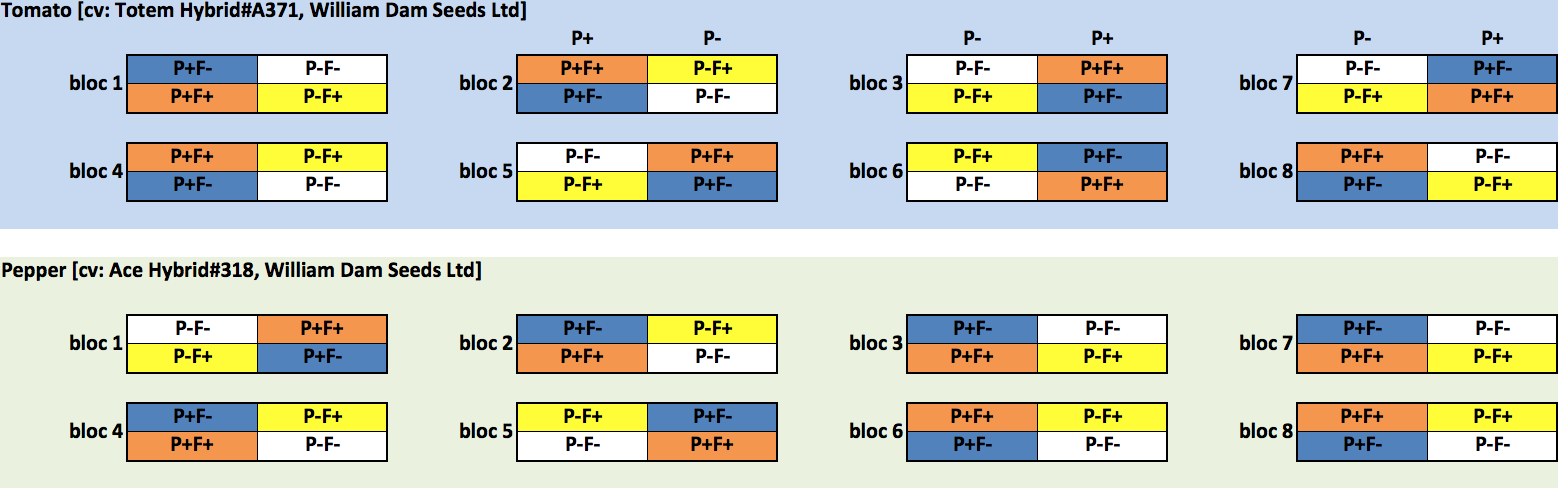
\includegraphics[width=5.20833in]{../figures/Figure1.png}\\
\textbf{Figure 1: experimental design}\\
\hspace*{0.333em}\\
Tomato plants were fertilized using multipurpose organic fertilizer
(pure hen manure, 18g per tray repeated every 4 weeks, 5-3-2) from
Acti-sol (Notre-Dame-du-Bon-Conseil, Qc, Canada) in addition to Stella
Maris® (3.5 ml per 1L, each tray received 250 ml, repeated every 2
weeks) for the duration of the experiment. Stella Maris® is a registered
trademark from Acadian Seaplants Ltd. (Darmouth, NS, Canada). It is
primarily composed of \emph{Ascophyllum nodosum} seaweed and is
advertized as a natural activator of the crops' own growth and defense
mechanisms to improve root growth and resist temperature, drought, and
salinity stress in order to maximize yield and crop qualities (ref.).
Pepper plants were fertilized using solely Stella Maris (3.5 ml per 1L,
each tray received 250 ml, repeated every 2 weeks) for the duration of
the experiment.\\
\hspace*{0.333em}\\
Thrips were managed with \emph{Neoseiulus cucumeris} (syn.
\emph{Amblyseius cucumeris}) (100 bags), Fungus gnat and thrips were
also controlled using predatory mite \emph{Gaeolaelaps gillespiei} (1L).
Plants were treated once a week with Oïdium Milstop.\\
\hspace*{0.333em}\\
\hspace*{0.333em}\\
\emph{Plant productivity}\\
At the end of the experiment, plant productivity was assessed by
measuring four different traits (fruit number, average fruit weight,
shoots fresh weight, roots fresh weight) on three plants chosen randomly
per tray (for each treatment {[}fertilization/control{]}, species
{[}tomato/pepper{]} and block {[}eight blocks{]}) for a total of 96
samples. In addition, both shoots and roots were dried in a 70 degrees
drying oven, anddry weights were measured after 48 hours. Together,
these traits are expected to represent well the plant overall
productivity (ref.).\\
\hspace*{0.333em}\\
\hspace*{0.333em}\\
\emph{Sample preparation, DNA extraction and High throughput
sequencing}\\
We sampled both the microbial and fungal communities from soil and root
samples. Soil DNA was extracted using XXX DNA isolation kit with Yg of
soil. Roots were first washed with sterile water and DNA was extracted
using XXX DNA isolation kit with Yg of root samples. Amplicon sequencing
targeting 16S rRNA gene (bacteria) and ITS (fungi) was performed on both
root and soil samples.\\
\hspace*{0.333em}\\
In order to target fungi, we used fungal primers ITS3\_KYO2
(5'-ACACTGACGACATGGTTCT ACAGATGAAGAACGYAGYRAA-3') and ITS4\_KYO3
(5'-TACGGTAGCAGAGACTT GGTCTCTBTTVCCKCTTCACTCG-3') to produce a final
amplicon size of 430bp (Toju \emph{et al.} 2012).\\
\hspace*{0.333em}\\
Bacterial primers 341F (5'-CCTACGGGNGGCWGCAG-3') and 805R
(5'-GACTACCAGGGTATC TAATC-3') producing a final amplicon size of
\textasciitilde{}464b and targeting specifically the bacterial V3-V4
region of the 16S ribosomal gene were chosen given that they has been
used extensively in high-throughput sequencing studies in a range of
environments (Hugerth \emph{et al.} 2014). This primer pair was shown to
be the least biased among 512 primer pairs evaluated in silico for
bacterial amplification (Klindworth \emph{et al.} 2012).\\
\hspace*{0.333em}\\
DNA samples were then barcoded, pooled and sequenced (2X300bp,
paired-end) using an Illumina MiSeq (San Diego, CA, USA) sequencer at
the Genome Quebec Innovation Centre (Montreal, Canada). Sequences were
demultiplexed by the sequencing facility (Genome Quebec Innovation
Centre) and further processed as described below.\\
\hspace*{0.333em}\\
\hspace*{0.333em}\\
\emph{Bioinformatics}\\
All bioinformatics, statistical, and graphic analyses further described
were performed in R 3.4.4 (R Core Team 2018) and detailed scripts are
available here (\url{https://github.com/seb951/Acadian_Seaplants}).\\
\hspace*{0.333em}\\
We used the R package dada2 (Callahan \emph{et al.} 2015) to infer
\emph{Amplicon Sequence Variants (ASVs)}. Dada2 offers accurate sample
inference from amplicon data with single-nucleotide resolution in an
open source (R) environments. Unlike the Operational Taxonomic Unit
(OTU) approach (e.g.~Schloss \emph{et al.} 2009, Caporaso \emph{et al.}
2010), ASV are not treated as cluster of sequences defined with an
\emph{ad hoc} sequence similarity threshold, thus allowing sequences and
abundance counts to be compared among studies (Callahan \emph{et al.}
2015).\\
\hspace*{0.333em}\\
First, sequences were trimmed following strict quality thresholds (see
parameter details in the accompanying R scripts). Following this, we
applied the error model algorithm of dada2 which incorporates quality
information after filtering, unlike other OTU based methods. Then
dereplication, sample inference, merging of paired end reads and removal
of chimera reads were performed in order to obtain a sequence (ASVs)
table of abundance per sample. Taxonomy was also assigned using the
Ribosomal Database Project (RDP) Naive Bayesian Classifier algorithm
from Wang \emph{et al.} (2007). Depending on support (minimum bootstrap
support of 80), we assigned taxonomy from Kingdom to species. We used
the silva database formatted for dada2 to infer bacterial taxa (Callahan
2018). We used the UNITE (2017) fasta release (including singletons) to
infer fungal taxa after formatting it to the dada2 format using a custom
R script. The dada2 pipeline was run on a multithreaded (48 CPUs)
computer infrastructure provided by Westgrid
(\url{https://www.westgrid.ca/support/systems/cedar}) and Compute Canada
(www.computecanada.ca). Note that the pipeline was run separately for
fungal-root, fungal-soil, bacteria-soil and bacteria-root samples given
the markedly different type of amplicons, taxa and error models of each
dataset. ~\\
\hspace*{0.333em}\\
\emph{Statistical analyses - plant productivity}\\
We tested for the effect of species (tomato vs pepper), fertilization
and their interaction on six plant productivity measures (fruit number,
average fruit weight, shoots fresh weight, roots fresh weight, shoots
dry weight, roots dry weight). We used linear mixed effect models (LMM)
in the R package NLME (Pinheiro \emph{et al.} 2017), which are more
appropriate than ANOVAs given the current block design (blocks and
replicates nested within a block were treated as random variables). All
six plant productivity measures were square root transformed in order to
help satisfy the assumption of normality of the residuals in the LMM
statistical framework.\\
\hspace*{0.333em}\\
\hspace*{0.333em}\\
\emph{Statistical analyses - microbial and fungal diversity}\\
We analysed separately fungal-root, fungal-soil, bacterial-root and
bacterial-soil ASV diversity. For each of these four datasets, we
removed samples that showed poor sequencing output and contained few
ASVs. In order to do this, we summed the abundance of all ASVs for each
sample (\(\sum_{i=1}^n ASV\)) and eliminated samples that had fewer that
the mean sum (\(\overline{\sum_{i=1}^n ASV}\)) - 4\(\sigma\) (four
standard deviations). In addition, we removed ASVs from our dataset that
were present in fewer than 5\% of the samples (less than 10 individuals
in the soil samples, and less than 5 in the root samples). This was done
to remove very rare ASVs which were unique to a block or replicate, but
not found in the majority of a treatment.\\
\hspace*{0.333em}\\
We then conducted community-based analyses looking at the effect of the
fertilization treatment on the abundance ASV taxa in the tomato and
pepper experiments. To reduce the complexity of the datasets, relative
abundance of all taxa were calculated per family using dplyr (Wickham
\emph{et al.} 2015). Barplots were drawn using ggplot2 (Hadley 2016) to
vizualize the communities. ASV (\(a\))-diversity was calculated for each
sample using the inverse Simpson diversity index in the R package VEGAN
(Oksanen \emph{et al.} 2013). The effect of fertilization treatment,
species (and planting for soil communities) were assessed using a linear
mixed-effect (LMM) model in the R package NLME (Pinheiro \emph{et al.}
2017), given the unbalanced, replicated block design. Alpha diversity
was log transformed in order to help satisfy the assumption of normality
of the residuals of the LMM statistical framework.\\
\hspace*{0.333em}\\
Using the community matrix data of ASVs abundance, we performed
PERmutational Multivariate ANalysis Of VAriance tests (PERMANOVA;
Anderson 2001) to identify relationships between the communities
according to the experimental design. ASV abundance data was
Hellinger-transformed and significance was assessed using 10,000
permutations in VEGAN (Oksanen \emph{et al.} 2013). Blocks and
replicates nested within blocks were factored as strata (blocks) in the
model.\\
\hspace*{0.333em}\\
We also performed constrained ordinations (CCAs) using
Hellinger-transformed ASV abundance data in VEGAN (Oksanen \emph{et al.}
2013) to visually assess the grouping of samples, ASVs and their
association with productivity variables. Data were analysed separately
for fungal-root, fungal-soil, bacterial-root and bacterial-soil, but
also according to species (tomato/pepper), given had analyses of
diversity showed that tomato and pepper were markedly different. This
gave a total of eight CCAs. Data were constrained based on four of the
productivity measures (fruit number, average fruits weight, shoots fresh
weight, roots fresh weight). We excluded the shoot \& root dry weights
as constraints to simplify the model, also given that they were highly
correlated with the fresh weigth already included as constraints
(\(r^2\)=0.98 and 0.76 for shoot dry/fresh weights and root dry/fresh
weights, respectively). ~\\
\hspace*{0.333em}\\
We then identified the ten ASVs most positively associated with the
productivity measures of fruit number, shoots fresh weight and roots
fresh weight from each constrained ordinations for a total of 40 fungal
and 40 bacterial candidates ASVs. We aligned sequences using the
Bioconductor R package decipher (Wright 2016) and build pairwise
distances matrices using a JC69 substitution models of DNA sequence
evolution (equal base frequencies, Jukes \& Cantor 1969) in phangorn
(Schliep 2010). Phylogenetic trees for bacteria and fungi were plotted
using ape (Paradis \emph{et al.} 2004). This permitted to identify if
similar candidate ASVs were found under different experimental
conditions (soil/root, pepper/tomato), thus reinforcing their role in
productivity increase, and decreasing the change that these are false
positive.\\
\hspace*{0.333em}\\
{[}A partition of the variation was also performed to assess how much of
the variation was explained by the soil and the vegetation
characteristics. I didn't include this in the end\ldots{}{]} ~

\newpage  

\section{RESULTS}\label{results}

\emph{productivity}\\
We tested the effect of the fertilization treatment on six different
measures of overall plant growth and productivity (fruit number, average
fruit weight, shoots fresh weight, roots fresh weight) for both tomato
and peppers. Fertilized plants grew better and this is apparent both
visually (Figure 2) and statistically (Figure 3). ~\\
\includegraphics[width=5.20833in]{../figures/productivity/Figure_2_photos_productivity.png}\\
\textbf{Figure 2: photos of plant productivity. From top left to bottom
right, fertilized pepper plants, pepper roots, pepper fruits and tomato
fruits and pictures to the left of the control plants.}\\
\hspace*{0.333em}\\
In fact, all six productivity measures significantly differed according
to species, and five of those were significantly different according to
the fertilization treatment. The only exception was the average fruit
weight which did not differ between fertilized and control plants (LMM,
\(F_{(1,69)}\) = 1.27, \emph{p}-value=0.26). However the model did
reveal a significant interaction between treatment and plant
(\(F_{(1,69)}\) = 9.6, \emph{p}-value=0.0028), such that when testing
only the pepper plants, the effect of fertilization on average fruit
weight was significantly higher in the fertilized pepper plants
(\(F_{(1,23)}\) = 10.84, \emph{p}-value=0.0032).\\
\hspace*{0.333em}\\
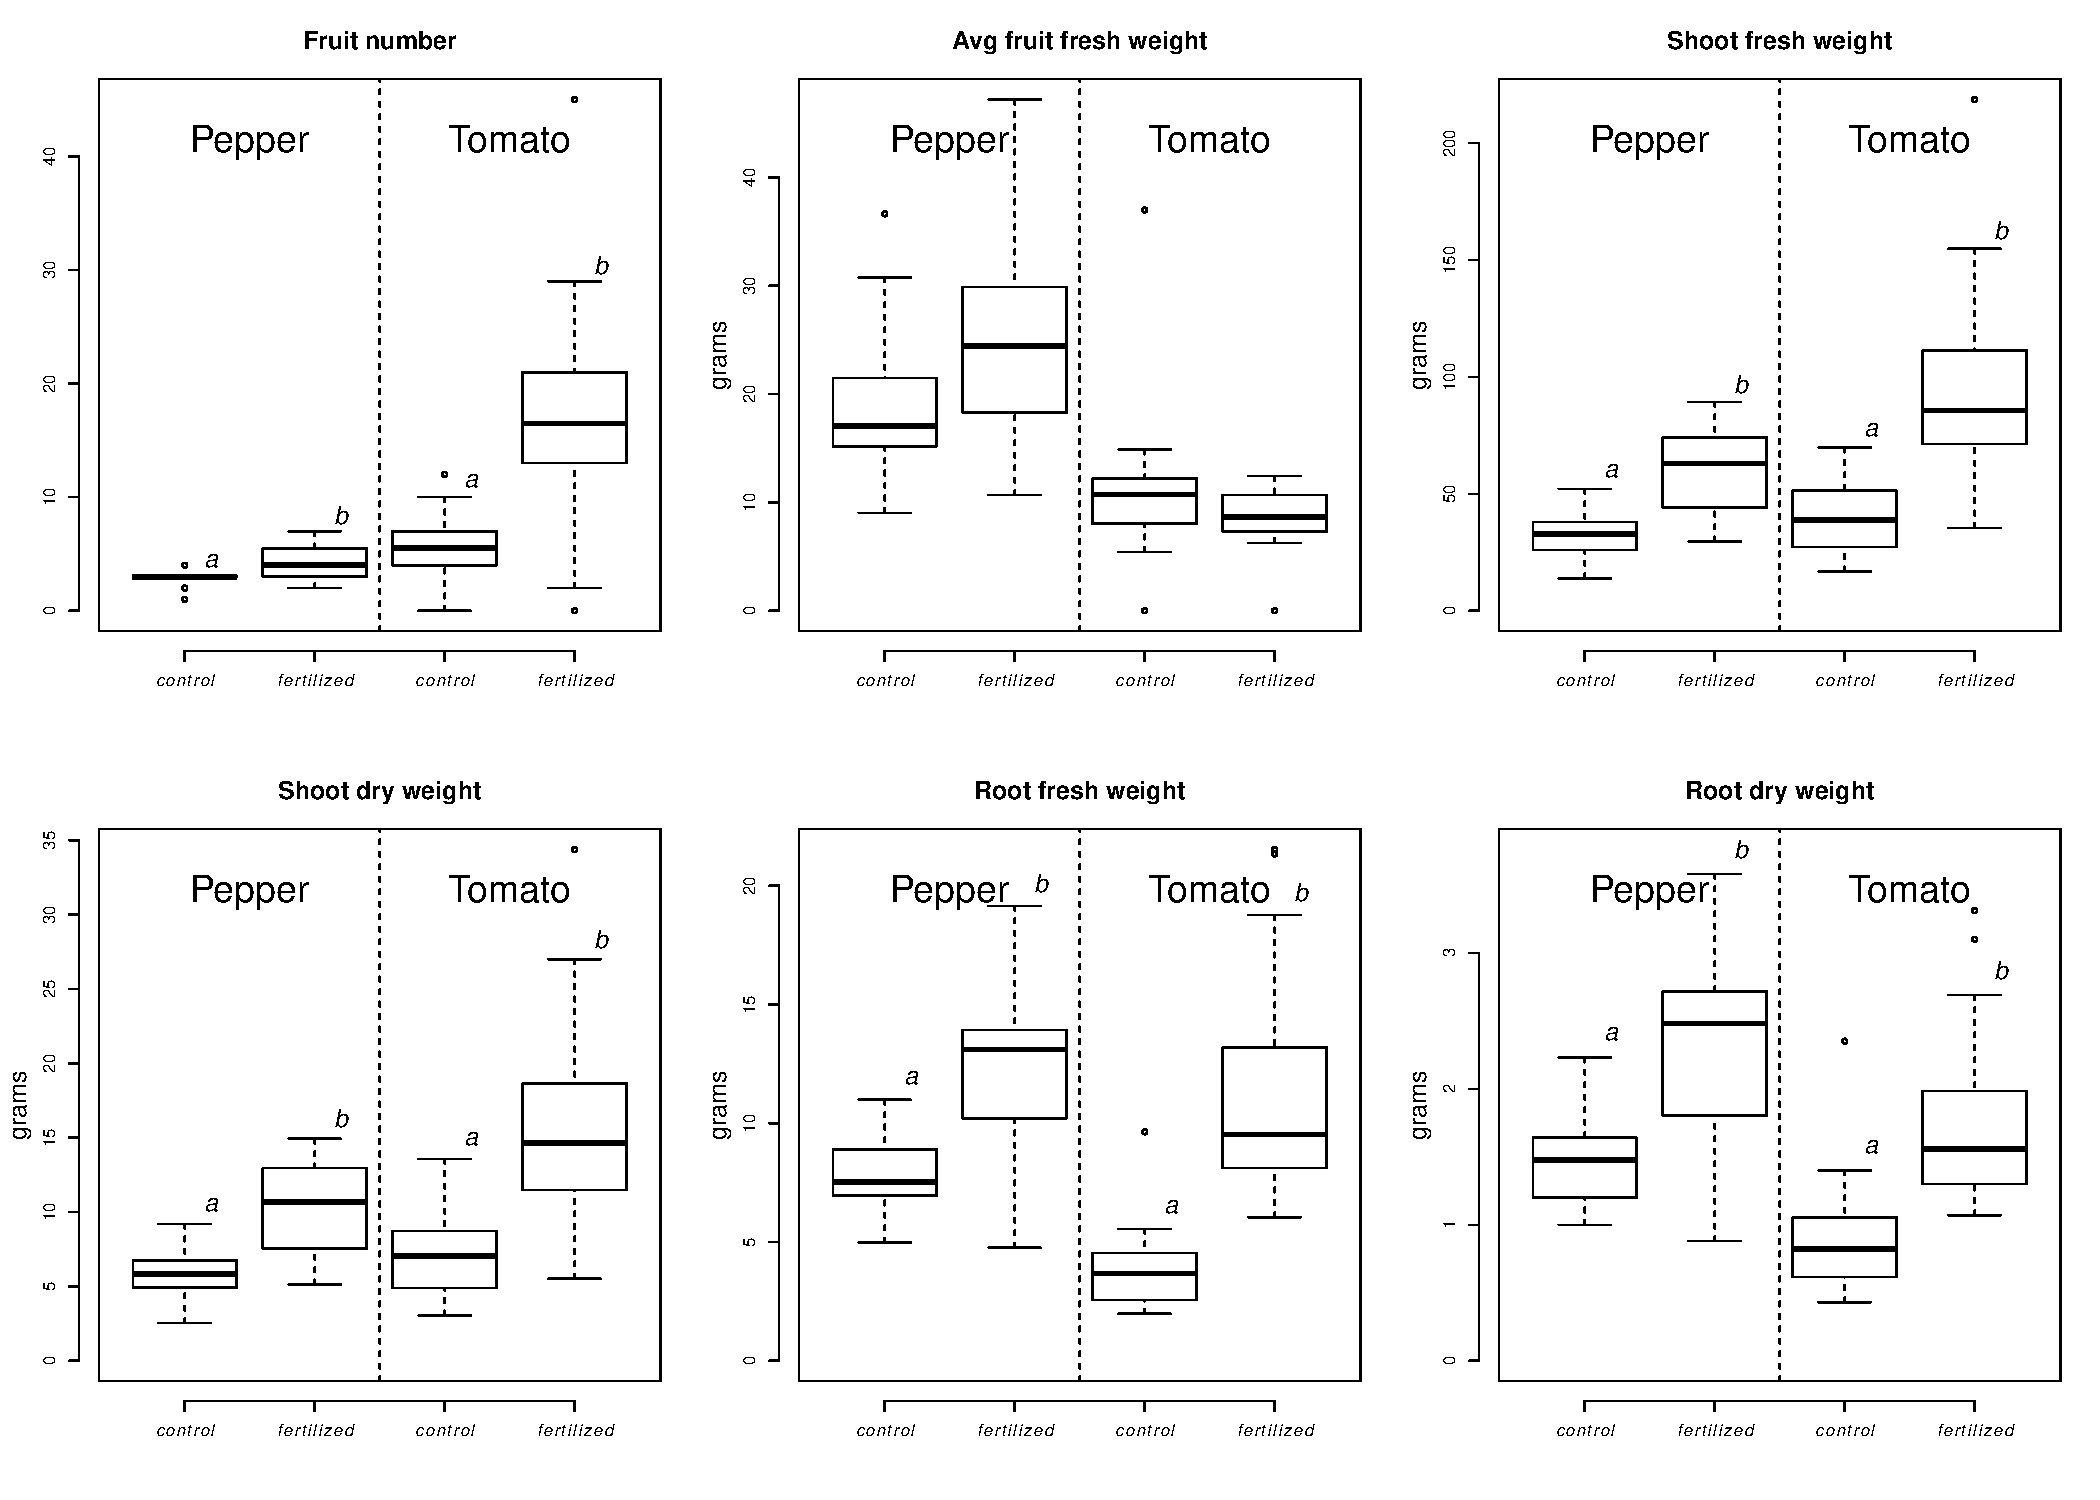
\includegraphics[width=6.25000in]{../figures/productivity/Figure_3_productivity.pdf}\\
\textbf{Figure 3: measures of plant productivity.}\\
\hspace*{0.333em}\\
\hspace*{0.333em}\\
\emph{Sequencing}\\
A total of 2.7 million paired-end raw reads were obtained for all
samples combined (976,000 for fungi-soil, 920,000 for fungi-root,
309,000 for bacteria-soil and 535,000 for bacteria-root, Table 2). Note
that sequencing samples were analysed separately for fungal-soil,
fungal-root, bacteria-soil and bacteria-root conditions. On average,
46,965 paired-end reads were obtained per sample, and after quality
filters were applied, including removing chimeras and paired-end reads
were merged, an average of 18,435 sequences remained. While 192 soil
samples for fungi and bacteria, and 92 root samples for fungi and
bacteria were sequenced, three fungi-soil samples, 13 fungi-root samples
and two bacteria-root samples were removed because they had to few
reads.\\
\hspace*{0.333em}\\
On average, 112 Amplicon Sequence Variants were identified per sample
(average of 163 fungal-soil ASV, 49 fungal-root ASVs, 112 bacterial-soil
ASVs and 122 bacterial-root ASVs). Many of those were unique to one of a
few samples (total number of 6,178 fungal-soil, 930 fungal-root, 10,120
bacterial-soil and 3,143 bacterial-roots ASVs). In fact, after quality
filtering ASVs that were found in fewer than 10\% of the samples, we
retained 418, 169, 206 and 250 ASVs and which comprised 91\%, 88\%, 50\%
and 85\% of all reads in the fungal soil, fungal roots, bacterial soil
and bacterial roots samples, respectively.\\
\hspace*{0.333em}\\
\hspace*{0.333em}

\begin{longtable}[]{@{}lrrrr@{}}
\caption{Sequencing and ASV summary}\tabularnewline
\toprule
& fungi\_soil & fungi\_root & bacteria\_soil &
bacteria\_root\tabularnewline
\midrule
\endfirsthead
\toprule
& fungi\_soil & fungi\_root & bacteria\_soil &
bacteria\_root\tabularnewline
\midrule
\endhead
Nb\_samples & 192 & 96 & 192 & 96\tabularnewline
Nb\_samples\_trimmed & 189 & 83 & 192 & 94\tabularnewline
Nb\_seq\_sumX10e3 & 976 & 309 & 920 & 535\tabularnewline
Nb\_seq\_mean & 51381 & 32208 & 47907 & 56365\tabularnewline
Nb\_seq\_mean\_filtered & 38045 & 14635 & 38287 & 46081\tabularnewline
Nb\_seq\_mean\_filt\_merged & 32014 & 13335 & 13780 &
41058\tabularnewline
Nb\_seq\_mean\_filt\_merg\_non\_chimeras & 24737 & 8505 & 12049 &
28451\tabularnewline
ASV\_persample & 163 & 49 & 112 & 122\tabularnewline
ASV\_sum & 6178 & 930 & 10120 & 3143\tabularnewline
ASV\_sum\_trimmed & 418 & 169 & 206 & 250\tabularnewline
\bottomrule
\end{longtable}

~\\
\hspace*{0.333em}\\
\emph{Root \& soil microbial and bacterial diversity}\\
We then analysed the whole community structure and report the relative
abundance of taxa (family) for the fungal-soil, fungal-root,
bacteria-soil and bacteria-root conditions (Figure 4). Fungal
communities were dominated but Nectriaceae, both the root and soil
samples. Bacterial root communities were largely dominated by the class
Oxyphotobacteria, but which could not be identified at the family level,
while Bacilaceae dominated to a lesser extent the soil communities.\\
\hspace*{0.333em}\\
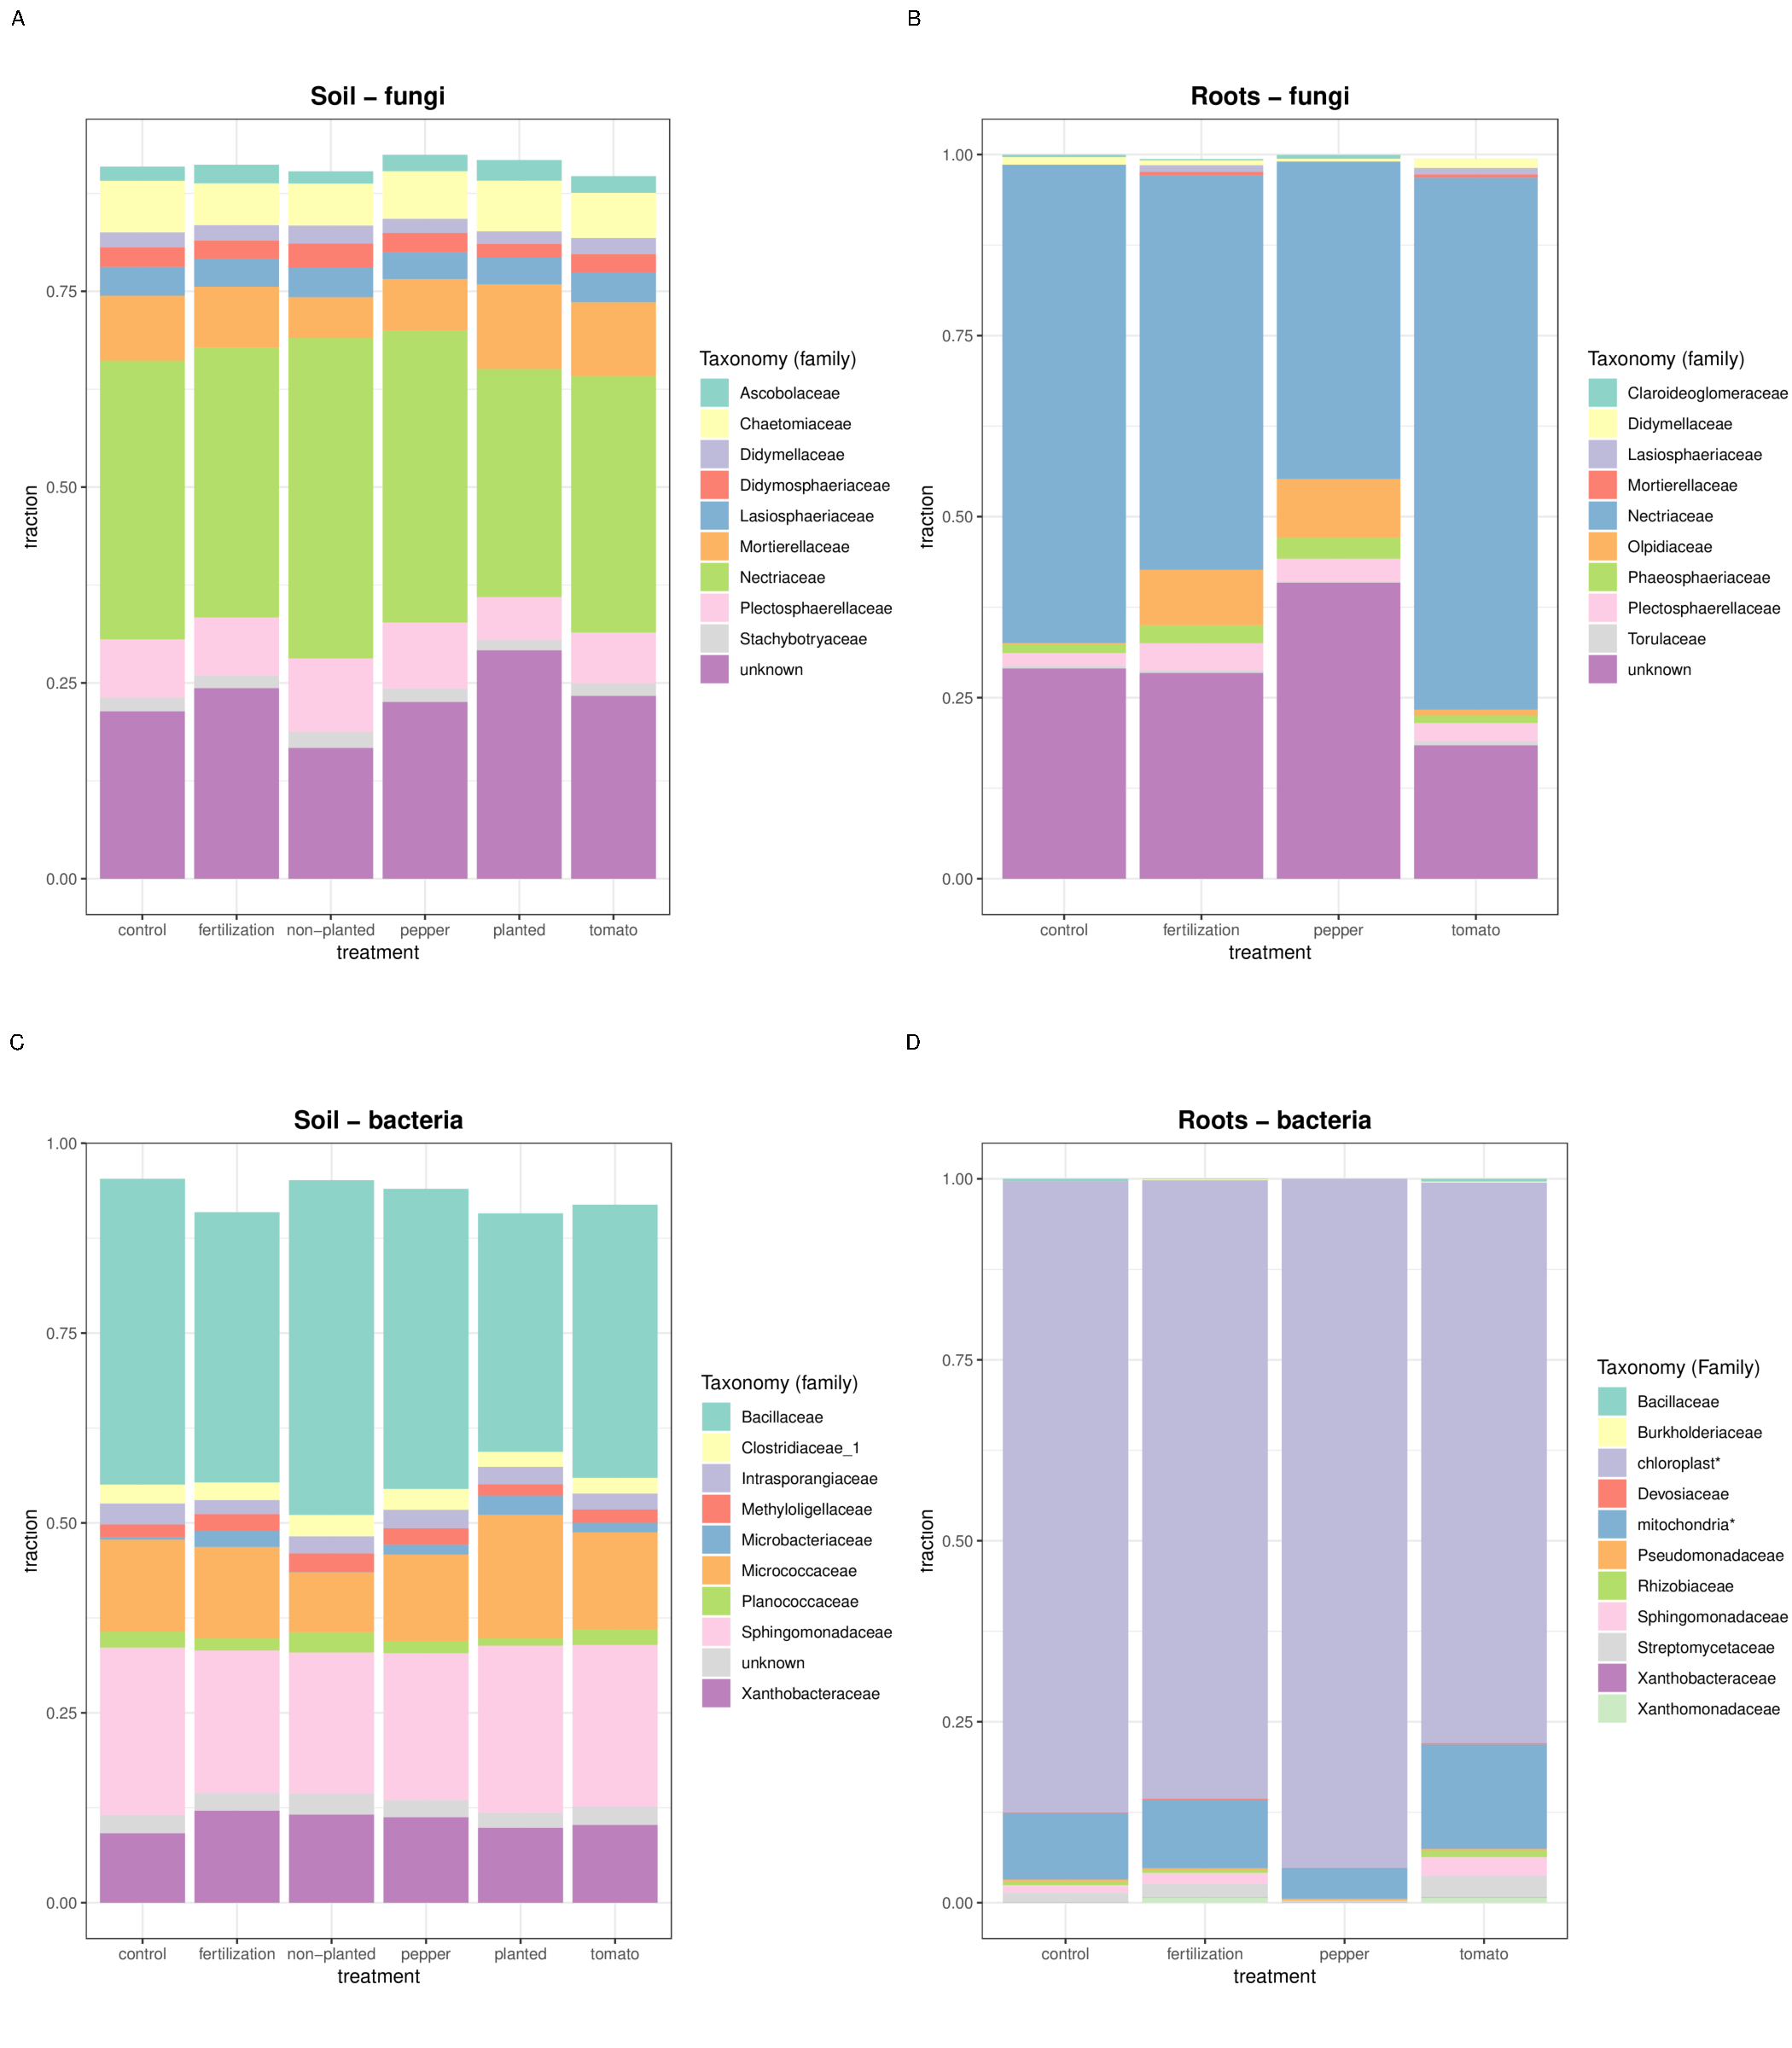
\includegraphics[width=7.29167in]{../figures/Figure4_barplots.pdf}\\
\textbf{Figure 4: Barplots.}\\
\hspace*{0.333em}\\
\hspace*{0.333em}\\
\emph{Local (\(a\)-diversity)}\\
The diversity of each site (\(a\)-diversity) was calculated for each
sample for each of the conditions (fungi-soil, fungi-root, bacteria-soil
and bacteria-root) and linear mixed effects models used to assess
significance (see Figure 5). In soils samples, fungal diversity differed
with respect to the fertilization (\(F_{(1,161)}\)=14.35,
\emph{p}-value\textless{}0.0001) and planting (\(F_{(1,161)}\)=41.00,
\emph{p}-value\textless{}0.0001) treatment, but not the species
(\(F_{(1,161)}\)=0.13, \emph{p}-value=0.72). In root samples, fungal
diversity differed with respect to the fertilization treatment
(\(F_{(1,56)}\)=13.56, \emph{p}-value=0.001), and the species
(\(F_{(1,56)}\)=74.31, \emph{p}-value=0.003). In soil samples, bacterial
diversity differed with respect to the fertilization treatment
(\(F_{(1,165)}\)=46.25, \emph{p}-value\textless{}0.0001), planting
(\(F_{(1,165)}\)=48.77, \emph{p}-value\textless{}0.0001) and species
(\(F_{(1,165)}\)=10.22, \emph{p}-value=0.002). In root samples,
bacterial diversity differed with respect to the fertilization treatment
(\(F_{(1,67)}\)=16.48, \emph{p}-value=0.0001), and the species
(\(F_{(1,67)}\)=523.42, \emph{p}-value\textless{}0.0001). ~\\
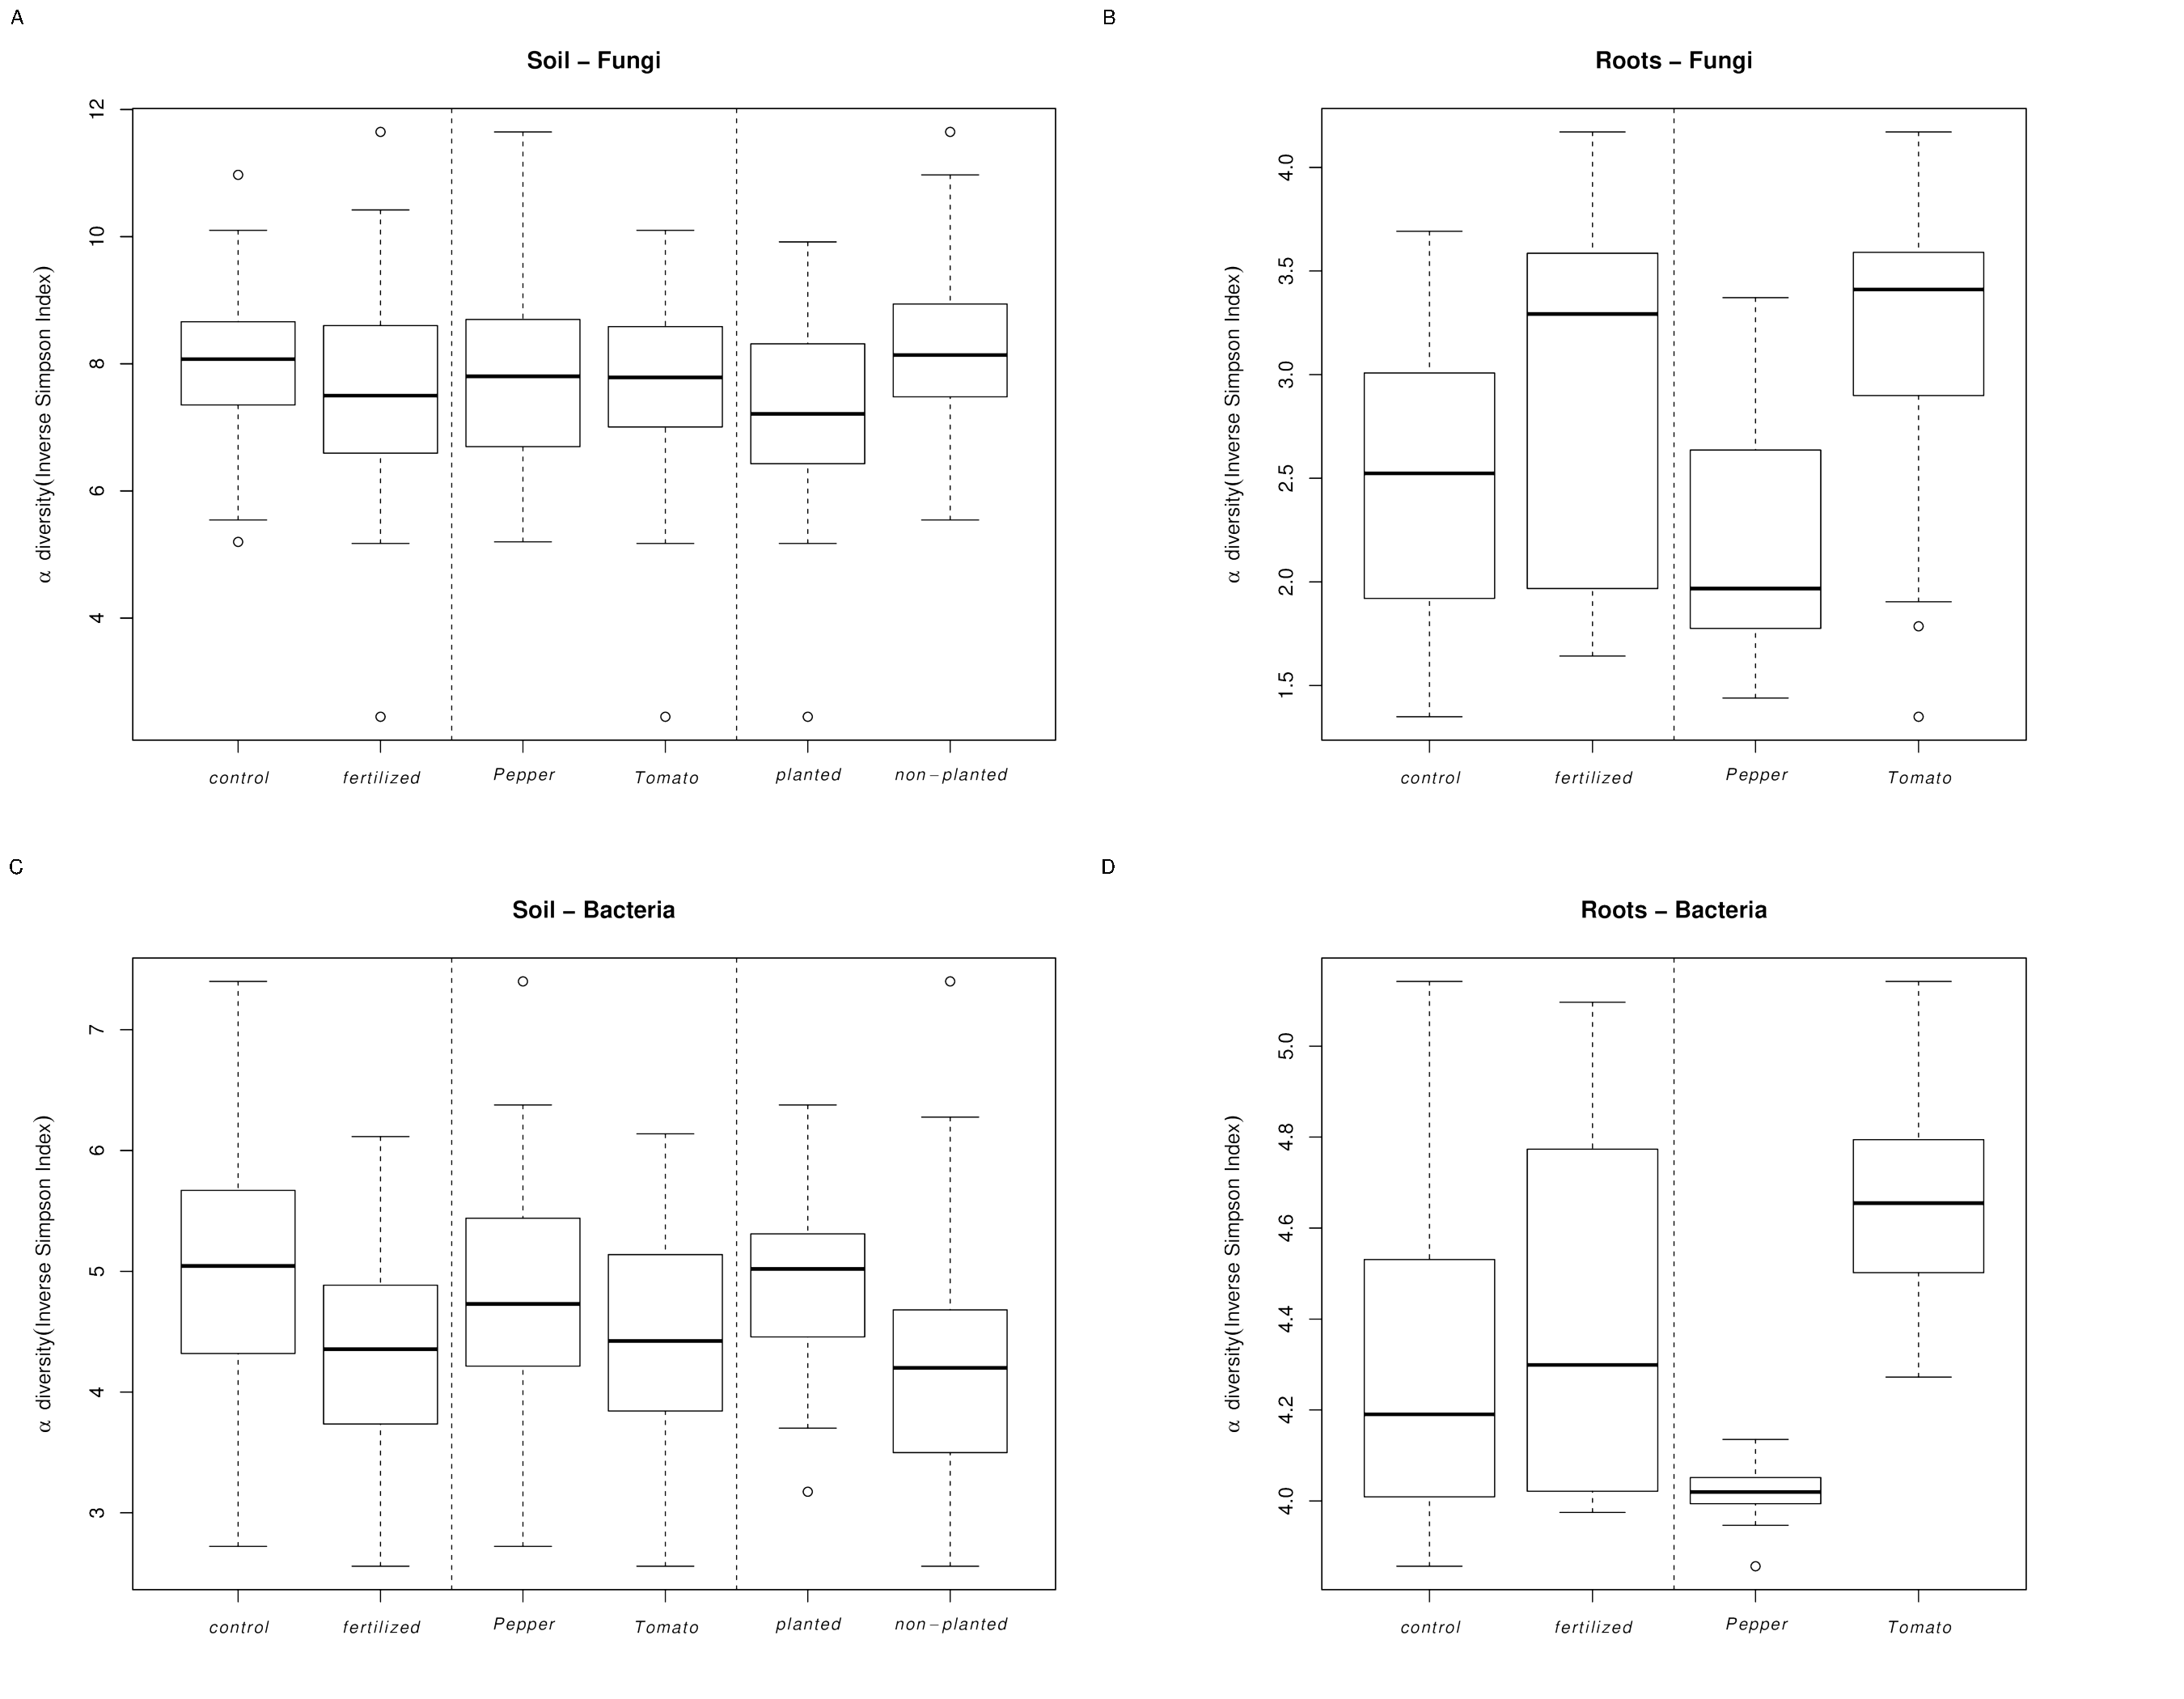
\includegraphics[width=6.25000in]{../figures/Figure5_alpha.pdf}\\
\textbf{Figure 5: Barplots.}\\
\hspace*{0.333em}\\
\hspace*{0.333em}\\
\emph{Differences in species composition among sites}\\
Using a PERMANOVA statistical framework, we identified that for all
conditions, communities differed with respect to the fertilization
treatment (Table 2). Soil fungal and bacterial communities differed the
most according to whether the tray was planted, while root communities
differed the most between tomato and pepper plants.\\
\hspace*{0.333em}

\begin{longtable}[]{@{}lllll@{}}
\caption{summary of PERMANOVAs*}\tabularnewline
\toprule
& fungi\_soil & fungi\_root & bacteria\_soil &
bacteria-root\tabularnewline
\midrule
\endfirsthead
\toprule
& fungi\_soil & fungi\_root & bacteria\_soil &
bacteria-root\tabularnewline
\midrule
\endhead
fertilization & 0.02 (4e-04) & 0.04 (0.0013) & 0.03 (1e-04) & 0.01
(0.0705)\tabularnewline
planted & 0.15 (1e-04) & NA & 0.06 (1e-04) & NA\tabularnewline
species & 0.02 (2e-04) & 0.2 (1e-04) & 0.01 (0.0032) & 0.42
(1e-04)\tabularnewline
fertilization:planted & 0.01 (0.008) & NA & 0.02 (1e-04) &
NA\tabularnewline
fertilization:species & 0.01 (0.0705) & 0.03 (0.0094) & 0.01 (0.002) &
0.01 (0.0973)\tabularnewline
planted:species & 0.01 (0.1597) & NA & 0.01 (0.1767) & NA\tabularnewline
fertilization:planted:species & 0 (0.7956) & NA & 0.01 (0.1179) &
NA\tabularnewline
\bottomrule
\end{longtable}

\emph{*R\textsuperscript{2} {[}percentage of variance explained by the
term in the model{]} and associated }p\emph{-values} ~\\
\hspace*{0.333em}\\
\emph{Constrained ordinations and candidate ASVs}\\
Constrained ordinations clearly indicated how fertilized samples
clustered together according to their fungal or bacterial communities
(Figure 6). It also shows how three of the constrain variables
(productivity measures of root fresh weight, shoots fresh weight and
fruit number) were associated with the fertilization treatment, while
average fruit weight behave differentially (in fact nearly orthogonally
to the other three constrains in most ordinations).\\
\hspace*{0.333em}\\
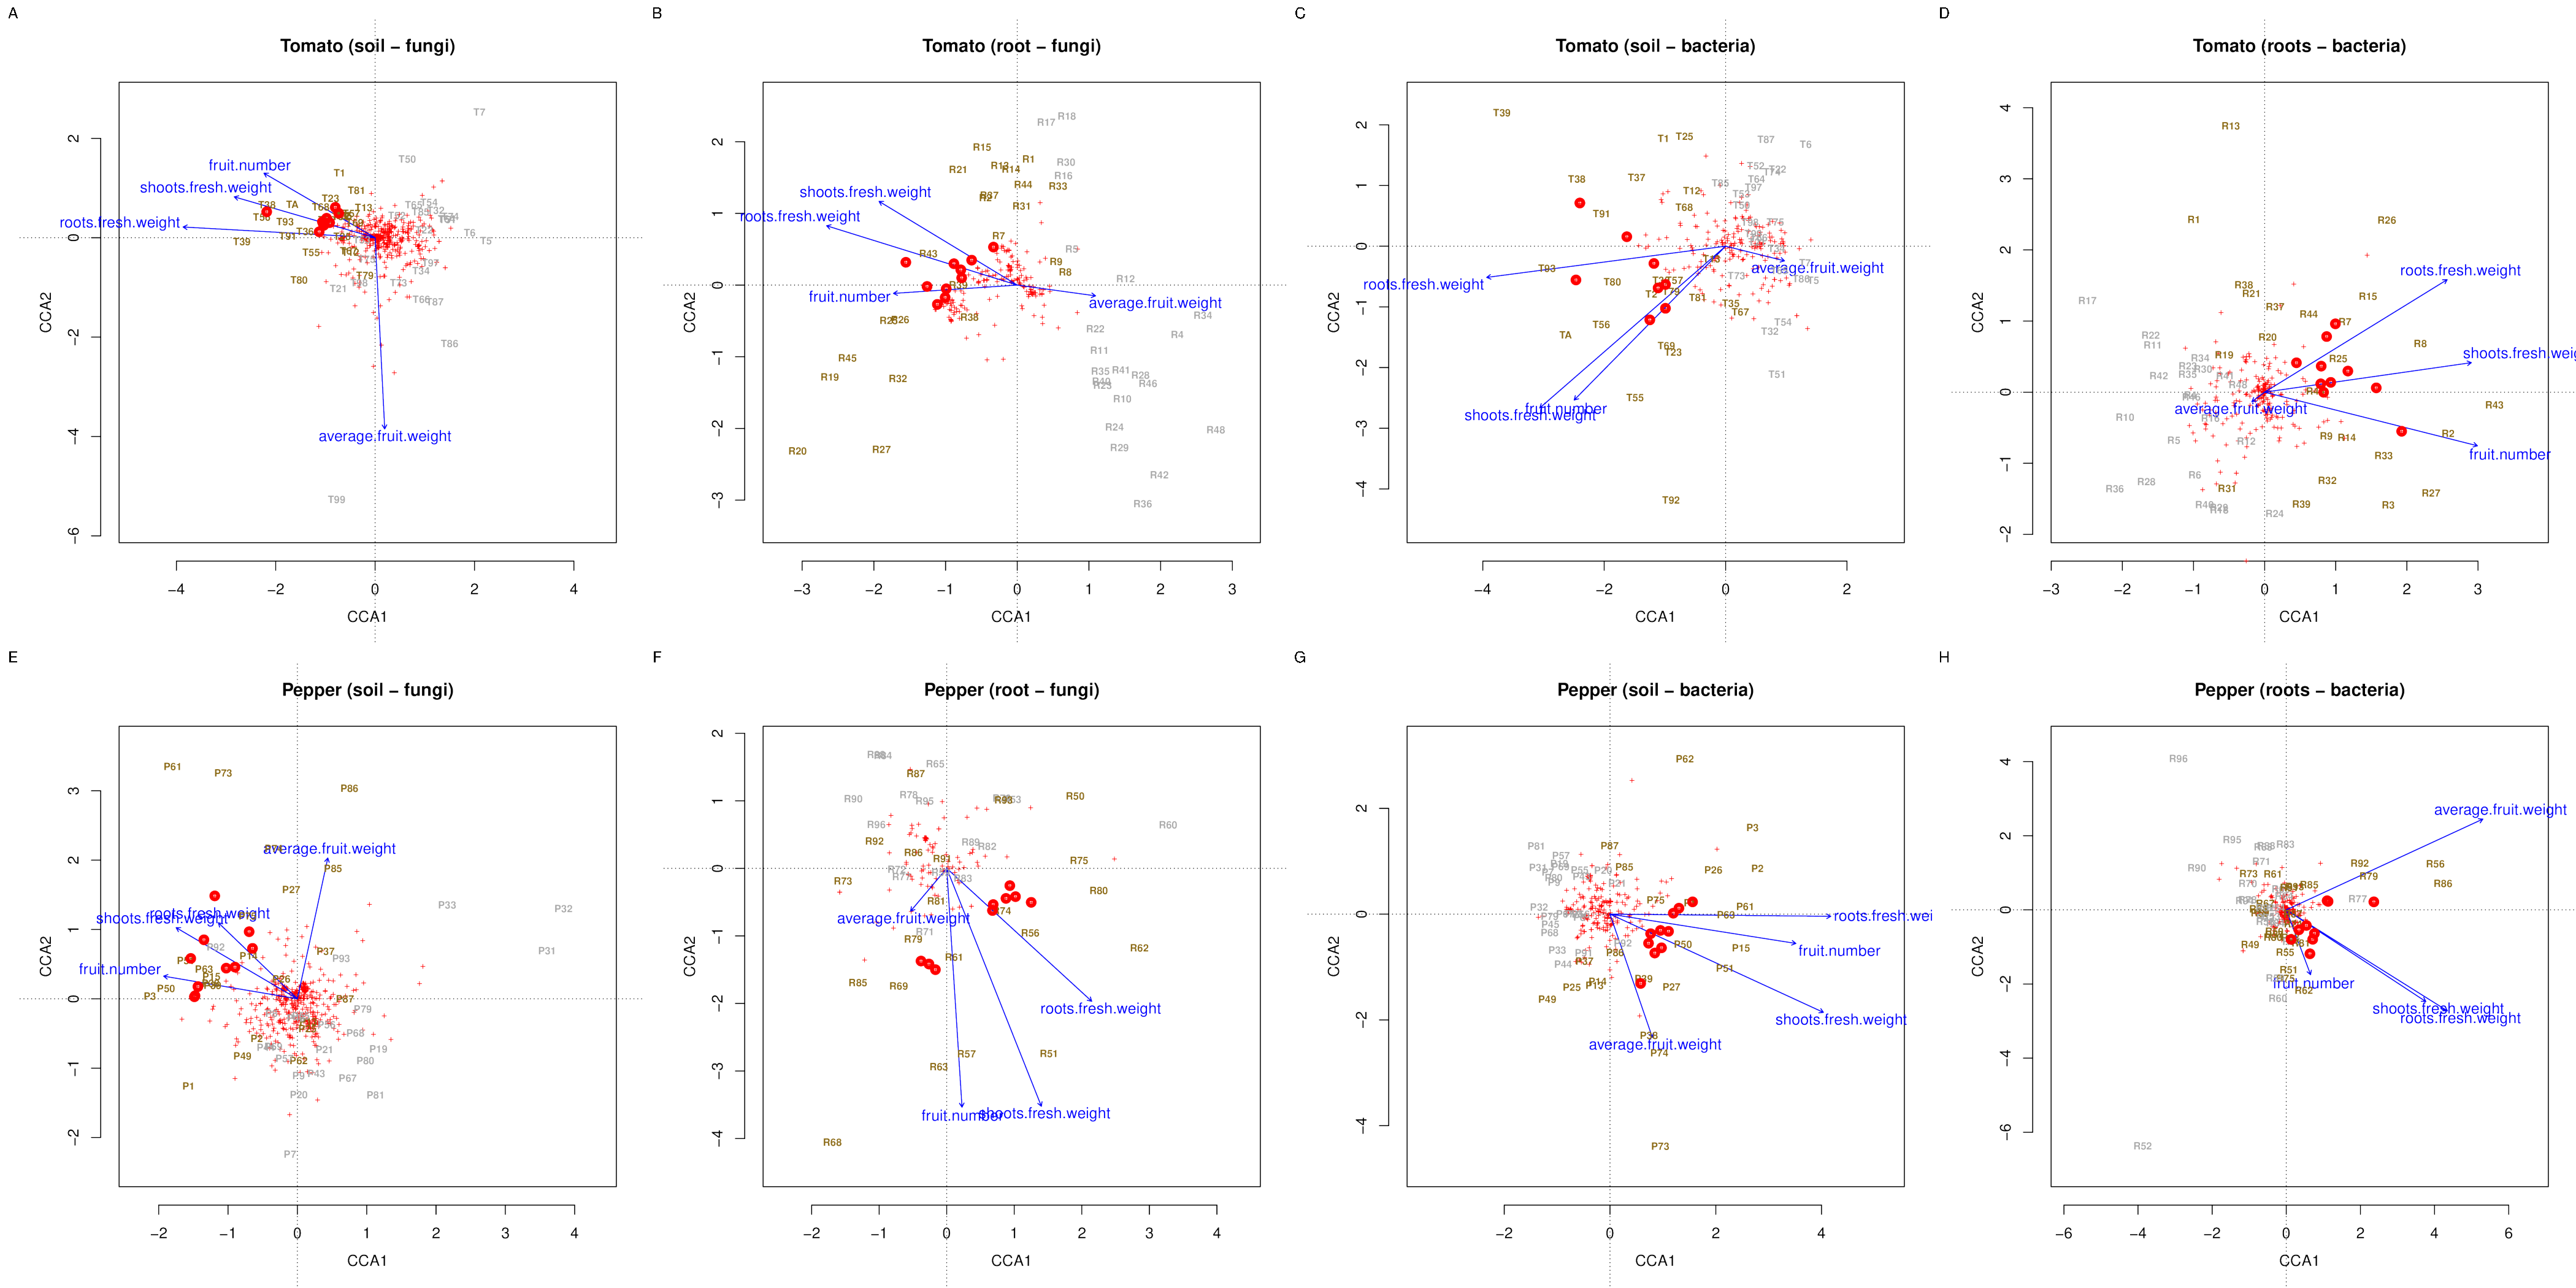
\includegraphics{../figures/Figure6_rda.pdf}\\
\textbf{Figure 6: rda.}\\
\hspace*{0.333em}\\
\hspace*{0.333em}\\
Next, we identified, for each ordination, the ten ASVs which were most
closely related to the three constrains which behave in a similar
fashion (productivity measures of root fresh weight, shoots fresh weight
and fruit number). These were considered as putative candidates which
may be most positively impacted (increase presence of the candidate) by
fertilization. We aligned the corresponding sequences for these eigthy
candidates (ten candidates * eight ordinations) ASVs in two seperate
alignments (one for fungi and one for bacterial ASVs), built distance
matrices and plotted neighbouring joining trees. In fungi, we identified
one cluster of ASVs taxonomically assigned to \emph{Olpidium brassicae}
that forms the majority of ASVs most closely related to productivity. In
addition, we identified seven closely related sequences closely related
to productivity in all both species and both root and soil.
Unfortunately, we could not assign taxonomy. SO WE BLASTED THESE
SEQUENCES TO OBTAIN MORE INFO ABOUT WHAT IT IS.

In bacteria, we identified a cluster of ten closely related sequences
taxonomically assigned to ``Chloroplast''. In fact this is most likely
the plant extract itself!!! Then we also have marine sps in the soil
(ASV267:Ilumatobacteraceae), which may come from the extract
itself\ldots{}

~\\
\hspace*{0.333em}\\
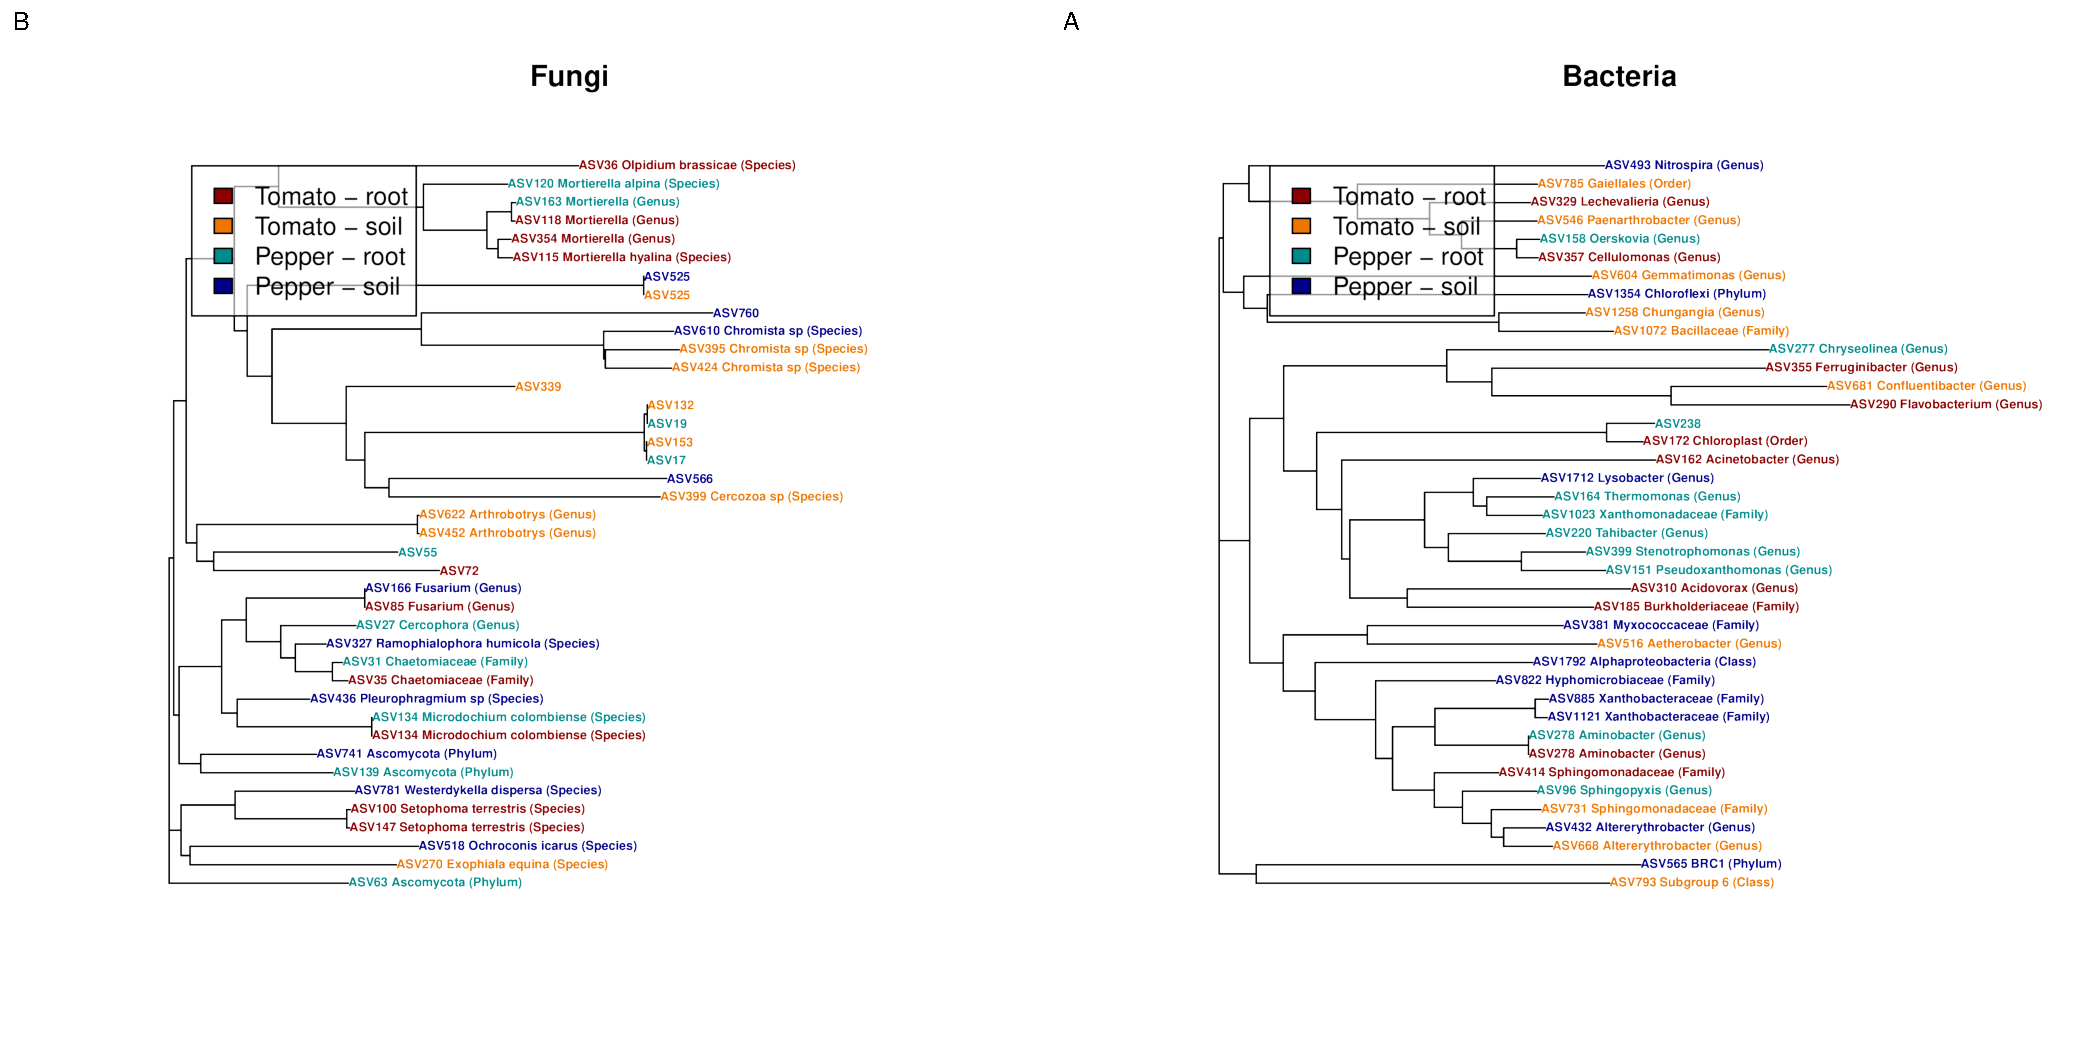
\includegraphics{../figures/Figure7_candidateASVs.pdf}\\
\textbf{Figure 7: Candidate trees} ~\\
\hspace*{0.333em}\\
\newpage   \#DISCUSSION\\
\newpage   \#REFERENCE\\
Anderson MJ. 2001. A new method for non-parametric multivariate analysis
of variance. Austral Ecology 26:32-46 Caporaso, J. Gregory, Justin
Kuczynski, Jesse Stombaugh, Kyle Bittinger, Frederic D. Bushman,
Elizabeth K. Costello, Noah Fierer et al. ``QIIME allows analysis of
high-throughput community sequencing data.'' Nature methods 7, no. 5
(2010): 335. ~\\
Craigie, J. S. 2011. Seaweed extract stimuli in plant science and
agriculture. J. Appl. Phycol. 23: 371 393 ~\\
silva for dada2: Silva taxonomic training data formatted for DADA2
(Silva version 132)). 10.5281/zenodo.1172783 ~\\
UNITE Community (2017): UNITE general FASTA release. Version 01.12.2017.
UNITE Community. \url{https://doi.org/10.15156/BIO/587475}
sh\_general\_release\_01.12.2017.zip ~\\
Wang, Q., Garrity, G. M., Tiedje, J. M., \& Cole, J. R. (2007). Naive
Bayesian classifier for rapid assignment of rRNA sequences into the new
bacterial taxonomy. Applied and environmental microbiology, 73(16),
5261-5267. ~\\
Klindworth, A., Pruesse, E., Schweer, T., Peplies, J., Quast, C., Horn,
M., \& Glöckner, F. O. (2013). Evaluation of general 16S ribosomal RNA
gene PCR primers for classical and next-generation sequencing-based
diversity studies. Nucleic acids research, 41(1), e1-e1. ~\\
Hugerth, Luisa W., Hugo A. Wefer, Sverker Lundin, Hedvig E. Jacobsson,
Mathilda Lindberg, Sandra Rodin, Lars Engstrand, and Anders F.
Andersson. ``DegePrime: a program for degenerate primer design for broad
taxonomic-range PCR for microbial ecology studies.'' Applied and
environmental microbiology (2014): AEM-01403. ~\\
Jukes TH and Cantor CR (1969). Evolution of Protein Molecules. New York:
Academic Press. 21--132.\\
\hspace*{0.333em}\\
Paradis, E., Claude, J., \& Strimmer, K. (2004). APE: analyses of
phylogenetics and evolution in R language. Bioinformatics, 20(2),
289-290. ~ Schloss, Patrick D., Sarah L. Westcott, Thomas Ryabin,
Justine R. Hall, Martin Hartmann, Emily B. Hollister, Ryan A. Lesniewski
et al. ``Introducing mothur: open-source, platform-independent,
community-supported software for describing and comparing microbial
communities.'' Applied and environmental microbiology 75, no. 23 (2009):
7537-7541. ~\\
Schliep, K. P. (2010). phangorn: phylogenetic analysis in R.
Bioinformatics, 27(4), 592-593. ~\\
Toju, H., Tanabe, A. S., Yamamoto, S., \& Sato, H. (2012). High-coverage
ITS primers for the DNA-based identification of ascomycetes and
basidiomycetes in environmental samples. PloS one, 7(7), e40863. ~\\
Wickham, H., Francois, R., Henry, L., \& Müller, K. (2015). dplyr: A
grammar of data manipulation. R package version 0.4, 3. ~\\
Wickham, Hadley. ggplot2: elegant graphics for data analysis. Springer,
2016. ~\\
Wright ES (2016). ``Using DECIPHER v2.0 to Analyze Big Biological
Sequence Data in R.'' The R Journal, 8(1), 352-359.




\newpage
\singlespacing 
\end{document}
